\documentclass[9pt]{beamer}
\usetheme{CambridgeUS}
\usepackage{xcolor}
\usepackage{geometry}
\usepackage{array}
\usepackage[export]{adjustbox}
\usepackage{comment}
\usepackage{caption}
\usepackage{subcaption}

\AtBeginSection[]
{
  \begin{frame}
    \frametitle{Table of Contents}
    \tableofcontents[currentsection]
  \end{frame}
}

\setbeamertemplate{footline}
{
  \leavevmode%
  \hbox{%
    \begin{beamercolorbox}[wd=.333333\paperwidth,ht=2.25ex,dp=1ex,center]{author in head/foot}%
      \usebeamerfont{author in head/foot}\insertshortauthor
    \end{beamercolorbox}%
    \begin{beamercolorbox}[wd=.333333\paperwidth,ht=2.25ex,dp=1ex,center]{title in head/foot}%
      \usebeamerfont{title in head/foot}\insertshortsubtitle
    \end{beamercolorbox}%
    \begin{beamercolorbox}[wd=.333333\paperwidth,ht=2.25ex,dp=1ex,right]{date in head/foot}%
      \usebeamerfont{date in head/foot}\insertshortdate{}\hspace*{2em}
      \usebeamertemplate{page number in head/foot}\hspace*{2ex}
    \end{beamercolorbox}
  }%
  \vskip0pt%
}

\title{Principles of Economics}
\subtitle{Discussion Session 8: GDP}
\author{Joe Wilske and Yuzhi Yao}
\institute{Boston College}
\date{\today}

\begin{document}

\frame{\titlepage}

\begin{frame}{Introduction to Macroeconomics}
        \begin{itemize}
        \item Microeconomics studies individual markets and agents.
        \vspace{5pt}
        \begin{itemize}
            \item The effect of a targeted tax on a particular good.
            \vspace{3pt}
            \item The effect of a minimum wage on a city's employment rate.
        \end{itemize}
        \vspace{5pt}
        \item Macroeconomics studies \textit{aggregated} markets and agents.
        \vspace{5pt}
        \begin{itemize}
            \item The effect of an income tax on an entire country's \textit{aggregate} demand.
            \vspace{3pt}
            \item The effect of new money creation on a country's \textit{aggregated} production.
        \end{itemize}
        \vspace{10pt}
        \item This requires new tools and types of models...
    \end{itemize}    
\end{frame}

\begin{frame}{Circular Flow Diagram}
\begin{columns}[c]
\begin{column}{0.5\textwidth}
    \begin{itemize}
        \item In micro, we tend to isolate a single direction of flow.
        \vspace{5pt}
        \begin{itemize}
            \item Firms sell goods to people, \textit{OR} \\people sell labor to firms.
            \vspace{5pt}
            \item ``Partial Equilibrium"
        \end{itemize}
        \vspace{5pt}
        \item In macro, we care about both directions of flow.
        \vspace{5pt}
        \begin{itemize}
            \item Firms sell goods to people, \textit{AND} \\people sell labor to firms.
            \vspace{5pt}
            \item ``General Equilibrium"
        \end{itemize}
    \end{itemize}
    \end{column}
    \begin{column}{0.5\textwidth}
        \centering
        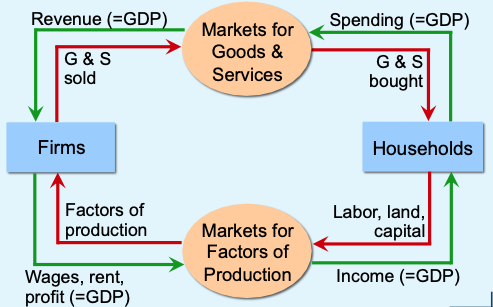
\includegraphics[width=\textwidth]{fig1.png}
    \end{column}
\end{columns}
\end{frame}

\begin{frame}{Circular Flow Diagram and GDP}
    \begin{itemize}
        \item Gross Domestic Product (GDP) is the value of everything produced in a country in a given time period -- usually a year.
        \vspace{3pt}
        \item ``Circular Flow" of the economy implies that we can calculate this in multiple ways:
        \vspace{3pt}
        \begin{itemize}
            \item \textbf{By income:} Add all wages, rents, interest, and profits earned within the country.
            \vspace{3pt}
            \item \textbf{By expenditure:} Add all expenditures made by people in the country.
        \end{itemize}
    \end{itemize}
    \vspace{5pt}
    \centering
    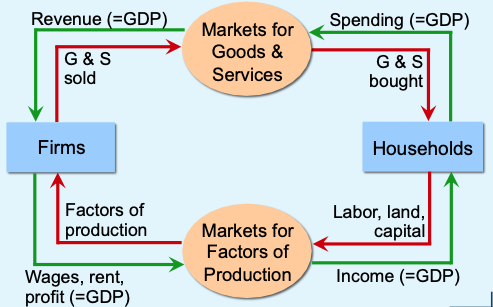
\includegraphics[width=.6\textwidth]{fig1.png}
\end{frame}

\begin{frame}{GDP Calculation}
    \begin{itemize}
        \item The \textbf{expenditures} approach is the most common:
    \end{itemize}
    \begin{align*}
        GDP = C + I + G + NX, \quad \text{where}
    \end{align*}
    \begin{align*}
        C &= \text{consumption}\\
        I &= \text{investment (includes change in inventories)}\\
        G &= \text{government (does not include transfer payments)}\\
        NX &= \text{net exports} = \text{exports} - \text{imports}
    \end{align*}
\end{frame}

\begin{frame}{Exercise 1: GDP Components}
    Suppose a country's expenditures are recorded as follows: 
    \begin{itemize}
        \item[-] Households’ spending on consumption = \$150 bn
        \item[-] Firms’ spending on capital goods = \$15 bn
        \item[-] Firms’ addition to inventories = \$8 bn
        \item[-] Government spending on services = \$20 bn
        \item[-] Government spending on social security = \$10 bn
        \item[-] Exports = \$10 bn
        \item[-] Imports = \$12 bn
    \end{itemize}
    What is the correct estimate of GDP?
    \vspace{1in}
\end{frame}

\begin{frame}{Exercise 1:GDP Components}
    Solution: 
    \begin{align*}
        C&=150\\
        I&=15+8=23\\
        G&=20\\
        NX&=10-12=-2\\
        GDP&=150+23+20-2=191
    \end{align*}
\end{frame}

\begin{frame}{Exercise 2: Calculate GDP}
    In May 2024, Michael in the US ordered a water bottle from an Italian seller's website. This bottle was made in Italy in 2023. How will this transaction affect: 
    \begin{itemize}
        \item[-] Italy GDP in 2023;
        \item[-] Italy GDP in 2024;
        \item[-] US GDP in 2023;
        \item[-] US GDP in 2024.
    \end{itemize}
    \vspace{1in}
\end{frame}

\begin{frame}{Exercise 2: Calculate GDP}
    Solution: 
    \begin{itemize}
        \item[-] Italy GDP in 2023: inventory increased 
        \item[-] Italy GDP in 2024: inventory decreased, export increased $\rightarrow$ not affected 
        \item[-] US GDP in 2023: not affected 
        \item[-] US GDP in 2024: import increased, consumption increased $\rightarrow$ not affected 
    \end{itemize}
\end{frame}

\begin{frame}{Exercise 3: Calculate GDP}
    Suppose an American clothing company imports machines from Japan for \$5,000. This company sells t-shirts they produced in the US for \$10,000 to their US customers. How much did the GDP of the US increase as a result of these transactions?
    \vspace{2in}
\end{frame}

\begin{frame}{Exercise 3: Calculate GDP}
    Solution: 
    \begin{align*}
        I&=5000\\
        NX&=0-5000=-5000\\
        C&=10000\\
        GDP&=5000-5000+10000=10000
    \end{align*}
\end{frame}

\begin{frame}{Accounting for Inflation}
    \begin{itemize}
        \item As the supply of money in the economy increases, so do the prices of goods.
        \vspace{5pt}
        \begin{itemize}
            \item Can loosely model this with supply and demand curves for dollars:\\
            \vspace{3pt}
            $S \uparrow$ means $P_{\text{dollar}} \downarrow$ means $P_{\text{goods}} \uparrow$
            \vspace{10pt}
        \end{itemize}
        \item Makes inter-year GDP comparisons difficult.
        \vspace{10pt}
        \item Did production increase, or did prices increase?
    \end{itemize}
\end{frame}

\begin{frame}{The GDP Deflator}
\begin{itemize}
    \item Choose a base year, 2020
    \vspace{3pt}
    \item Choose a year to compare, 2021
    \vspace{3pt}
    \item \textbf{Nominal GDP} of 2021 is the raw GDP calculation for the year ($C+I+G+NX$).
    \vspace{3pt}
    \begin{itemize}
        \item Use 2021 quantities and 2021 prices.
    \end{itemize}
    \vspace{3pt}
    \item \textbf{Real GDP} of 2021 is the inflation-adjusted GDP calculation.
    \vspace{3pt}
    \begin{itemize}
        \item Use 2021 quantities and 2020 prices.
    \end{itemize}
    \vspace{3pt}
    \item The \textbf{GDP Deflator} benchmarks the difference between \textbf{nominal} and \textbf{real} GDP:
    \end{itemize}
    \vspace{10pt}
    \begin{equation*}
        \text{Deflator 2020} = 100, \quad \quad \quad \quad \quad \text{Deflator 2021} = \frac{\text{Nominal 2021}}{\text{Real 2021}} \times 100
    \end{equation*}
    \begin{itemize}
        \item The \textbf{inflation rate} -- the rate of price increase -- is the percent change in the deflator from the previous year:
        \vspace{10pt}
    \end{itemize}
    \[
    \text{Inflation 2021} = \frac{\text{Deflator 2021} - \text{Deflator 2020}}{\text{Deflator 2020}} \times 100\%
    \]
\end{frame}

\begin{frame}{Exercise 4: GDP Deflator and Inflation Rate}
    Suppose an economy produces only green eggs and ham. Quantities and prices of these goods for the last several years are shown in the following table. The base year is 2015.
    \begin{table}[]
    \centering
    \begin{tabular}{ccccc}
    \hline
    Price & \multicolumn{2}{c}{Eggs} & \multicolumn{2}{c}{Ham}\\
         & Price & Quantity & Price & Quantity \\
    \hline
    2015 & 3 & 200 & 6 & 150 \\
    2016 & 3 & 250 & 7 & 200 \\
    2017 & 4 & 300 & 8 & 220 \\
    2018 & 5 & 350 & 7 & 120 \\
    \hline
    \end{tabular}
\end{table}
    \begin{enumerate}
        \item Calculate the GDP deflator in 2018.
        \item Calculate the inflation rate in 2018.
    \end{enumerate}   
    \vspace{1in}
\end{frame}

\begin{frame}{Exercise 4: GDP Deflator, CPI, and Inflation Rate}
    Solution:
    \begin{enumerate}
        \item GDP deflator in 2018 is 146.33
        \item GDP deflator in 2017 is 133.33; inflation rate in 2018 is 9.75\%.
    \end{enumerate}
\end{frame}


%%%%%%%%%%%%%%%%%%%%%%%%%%%%%%%%%%%%%%%%%%%%%%%%%%%%%%%%%%%%%%%%%%%%%%%%%%%%%%% For reference %%%
%%%%%%%%%%%%%%%%%%%%%%%%%%%%%%%%%%%%%%%%%%%%%%%%%%%%%%%%%%%%%%%%%%%%%%%%%%%%
\begin{comment}
\begin{frame}{Exercise 1: Calculate GDP}
    Suppose a cereal maker's finances for 2022 were as follows:
    \begin{itemize}
        \item[-] Wages: \$50000
        \item[-] Profits: \$10000
        \item[-] Expenditures on new machines: \$5000
        \item[-] Usage of ingredients bought last year: \$2000
    \end{itemize}
    What was the contribution to the GDP of this cereal maker in 2022? (\textit{Hint: use the circular-flow diagram.})
    \begin{figure}
        \centering
        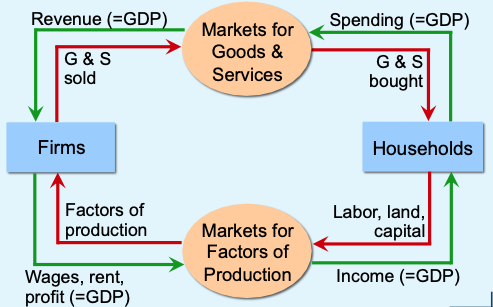
\includegraphics[scale=0.35]{fig1.png}
    \end{figure}
\end{frame}

\begin{frame}{Exercise 1: Calculate GDP}
    Solution: $GDP = 50000+10000+5000=65000$
\end{frame}
\end{comment}
\end{document}
